\chapter{\textsc{Unit� centrale}}

L'unit� centrale ou CPU et le coeur du microcontr�leur. Elle effectue des op�ration �l�mentaires sur des donn�es ou sur des adresses.


\section{Principes}

Un processeur se d�compose en deux unit� fondamentales: i) une unit� de contr�le et ii) une unit� de traitement  (fig. \ref{fig:cpu}). L'unit� de contr�le d�code les instructions et pilote le chemin de donn�es qui ex�cute les op�rations. Le pilote du chemin de donn�es s'appelle le s�quenceur, il communique avec le chemin de donn�es � l'aide de signaux de commande et re�ois des informations sur son �tat.

\begin{figure}[htb]
  \centering
  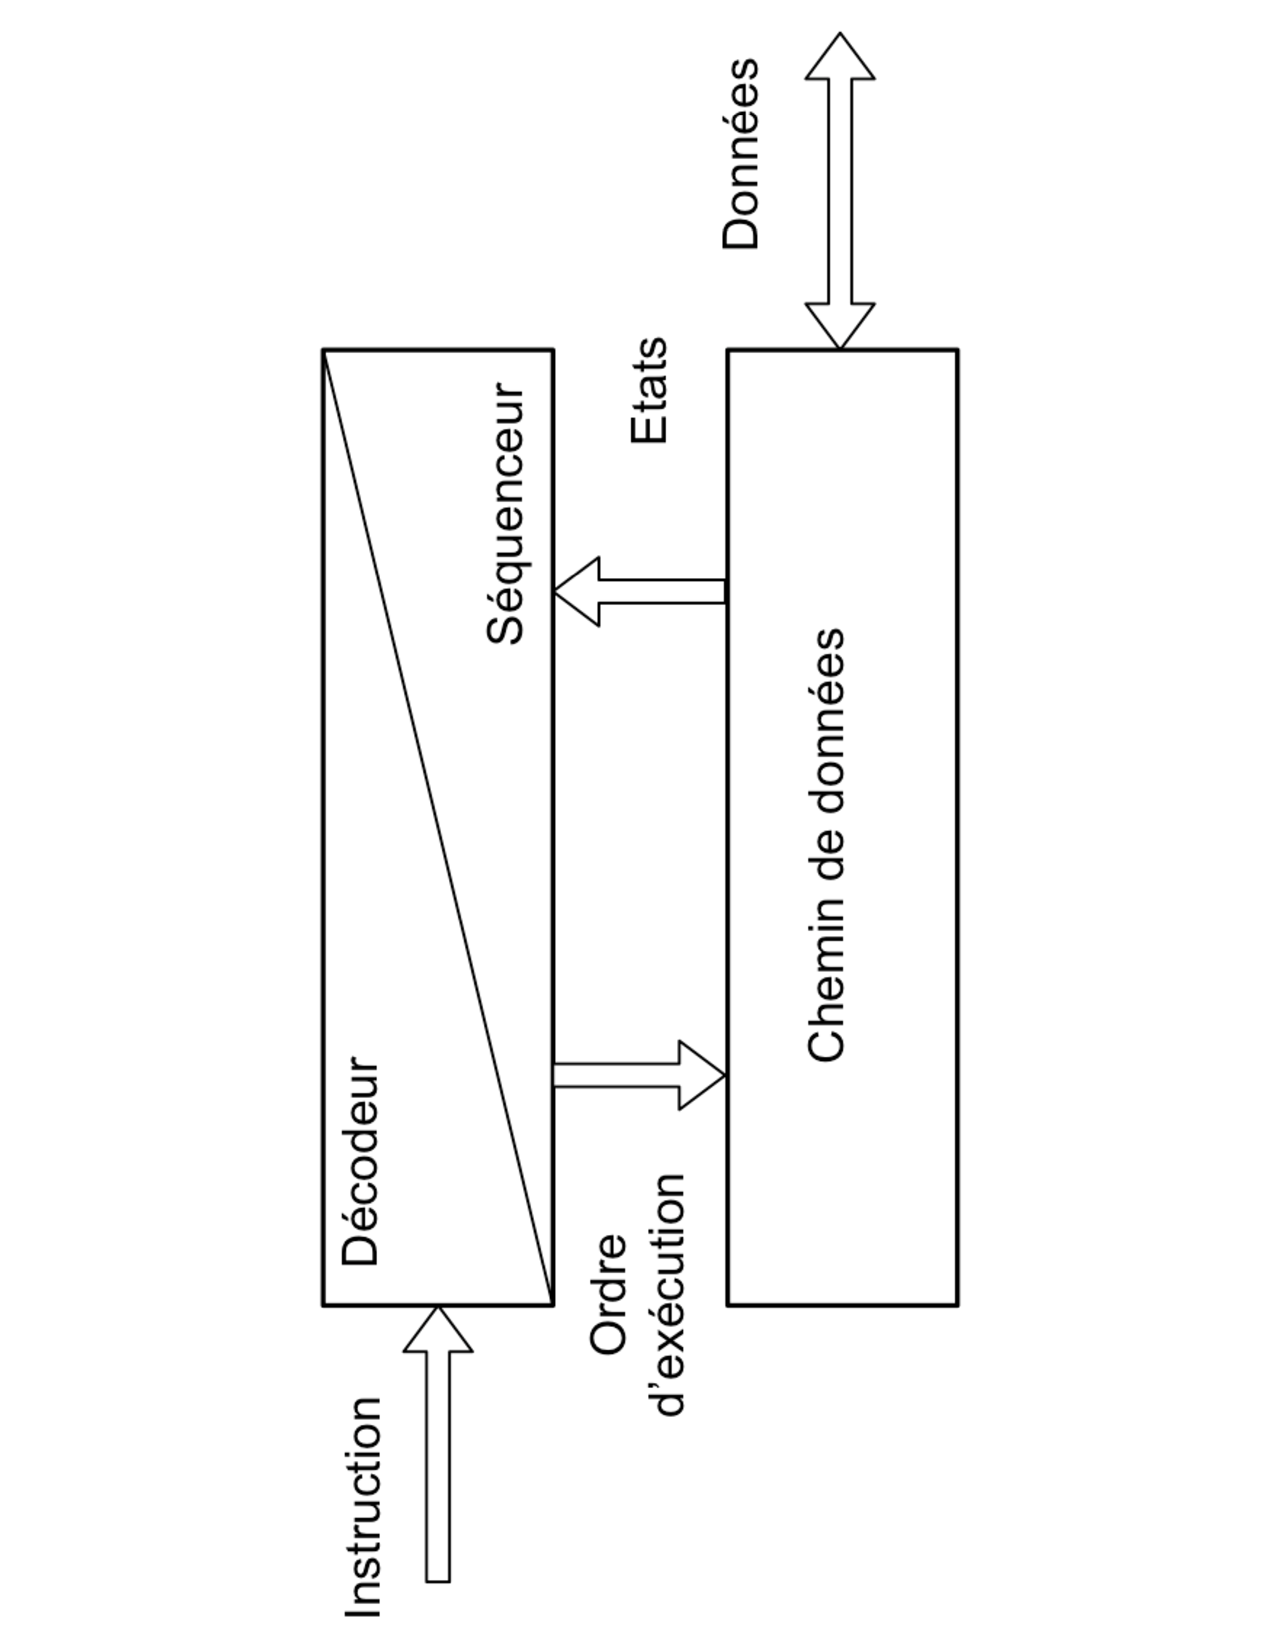
\includegraphics[angle=270, width=12cm]{./Figures/cpu/cpu.pdf}
  \rule{35em}{0.5pt}
  \caption[cpu]{Principe de fonctionnement de l'unit� centrale}
  \label{fig:cpu}
\end{figure}

Le s�quenceur est aussi responsable d'amener et de stocker des donn�es dans la m�moire. On constate que le processeur � besoin de deux types d'information, les instructions et les donn�es. Il y a donc deux possibilit�s, l'une ou l'on stock les deux informations dans une seule m�moire et l'autre ou on utilise deux m�moires s�par�es. Ce choix � provoqu� une distinction une importante en architecture des processeurs qu'on a nomm� Von Neumann et Harvard.

\subsection{Architecture de Von Neumann}

\subsection{Architecture de Harvard}


%\newpage 
\section{Cycles des instructions}


\subsection{Recherche de l'instruction}
%\newpage 
\subsection{D�codage de l'instruction}
%\newpage 
\subsection{Recherche des op�randes}
%\newpage 
\subsection{Ex�cution de l'instruction}
%\newpage 
\subsection{�criture du r�sultat}

%\newpage 
\section{S�quenceur des instructions}

%\newpage 
\section{Pipeline des unit� de calcul}

\section{Processeur super scalaire}